\subsection{Configuration Management Plan}
This software project consists of 5 official documents including SRS, SPMP, SDD, Testing report and User Manuel), meeting agenda and minutes, and software for operating EV3 robot. All these configuration items’ standards are developed by documentation manager and monitored by quality manager. All team members are responsible for following this configuration standard during the whole project life cycle. The detail of software and testing components will be mentioned in SDD document and testing report.

\subsection{GitHub Repository structure and Configuration control}
The repository structure is built based on the component of the project. The highest level of repository is Code and Documentation. 
\begin{itemize}
	\item \texttt{\detokenize{...\2017-S2-SEP-PG29\Documentation}}
	\item \texttt{\detokenize{...\2017-S2-SEP-PG29\Code}}
\end{itemize}
The detail GitHub Repository structure is shown on fig.3.

\begin{figure}[H]
	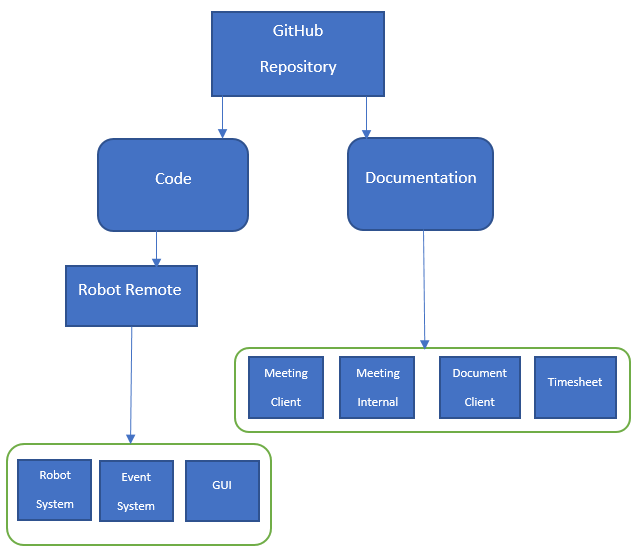
\includegraphics[width=\linewidth]{GIT.png}  % created using www.draw.io
	\caption{GITHUB repository}
	\label{fig:GITHUB repository}				
\end{figure}

There are three configuration directories which have special control for team members to edit. The Software components are not included in this section and will be discussed in detail on SDD document.\\
The lists of configuration control are shown as below:\\

\textbf{Library control:}\\
This library directory is for development purpose. There shall allow to store jar file only. No other file format is allowed. Team members are require to get the approval from development manager to add new jar file.\\ 
\begin{itemize}
	\item \texttt{\detokenize{...\Code\UiRemote\lib}}
\end{itemize}
\textbf{Media control:}\\
Those directory contain png file only. No other file format is allowed. Team members can feel free to add any png file for development or development purpose. Team members shall commit the change with proper message to indicate which files they are added.

\begin{itemize}
	\item \texttt{\detokenize{...Code\UiRemote\src\RobotRemote\UI\Views}}
	\item \texttt{\detokenize{...Documentation\Views}}
\end{itemize} 
\textbf{Documentation control:}\\
Those directories contain tex and pdf file only. Team members are not allowed to add any file in those directories.
Only documentation manager can add new file to those directories

\begin{itemize}
	\item \texttt{\detokenize{...Documentation\SRS}}
	\item \texttt{\detokenize{...Documentation\SPMP}}
	\item \texttt{\detokenize{...Documentation\SDD}}
\end{itemize}

\subsection{Configuration Naming System and version control}
Any draft of configuration items shall be followed as below naming standards:
\begin{itemize}
	\item \texttt{\detokenize{<Title>_<version>.<extension>}}\\
      		\texttt{\detokenize{For examples: SRS_v0.9.tex}}
	\item The Final version is v1.0. The draft version will be named as v0.1-v0.9.
	\item The modified date for each sub-version shall be mentioned in revision history table which is included into documents.\\
\end{itemize}

The examples of revision history for SRS-v0.9.tex is shown on Table2 :\\

\begin{table}[]
	\centering
	\caption{Revision history}
	\label{my-label}
	\begin{tabular}{|l|l|l|l|}
		\hline
		Name      & Date      & Version & Summary of Changes           \\ \hline
		1st Draft & 21/8/2017 & 0.9.1   & Initial Draft                \\ \hline
		2nd Draft & 22/8/2017 & 0.9.2   & Identification numbers added \\ \hline
	\end{tabular}
\end{table}


The revision table for final version shall include all the change for each version. After final version released, any change is required a change request which is mentioned in section 8.3.\\


The meeting agenda and meeting minutes shall follow as below naming system:\\
\texttt{\detokenize{<Title>_<Type>_<week>.<extension>}}\\
\begin{itemize}
\item Title: Agenda or Minutes
\item Type: Client or Internal
\end{itemize}
\texttt{\detokenize{For example: agenda_client_week3.tex, minutes_internal_week3.tex}} \\\\
Usually, there are only one client meeting and internal group meeting per week. If there are any emergency meeting, the date should be included.\\\\
\texttt{\detokenize{For example: agenda_internal_week3_17082017.tex}}\\
\texttt{\detokenize{The date format shall be <days><months><year>}}\\
\subsection{Change request handling}
There are two types change request handling. Documentation and Software change request handling.\\\\
\textbf{Documentation:}\\
The Documents will be divided by documentation manager into difference sub-tasks for each team member to edit their own parts. 
\begin{itemize}
\item Team members can make any change on their own part before the final version release. 

\item Team members is required to edit the revision table to record their change on the document. 

\item The documentation review meeting will be held by documentation manager to review all the changes on the document before releasing final version.

\item The change on Final version's document is not allowed without discussion in another new review meeting. 
\end{itemize}
\textbf{Software:}
\begin{itemize}
\item Team member must need to create new branch in github repository to make a change or add new function on software. 
\item The change on this branch must not affect master branch.
\item Regular software review meeting will be held by development manager to review all the team member’s work and discuss the potential issue before merging the work to master branch.
\end{itemize}